%\documentclass[]{book}
%\usepackage[subpreambles=false]{standalone}

%%%%%%%%%%%%%%%%%%%%%%%%%%%
% Silence warning messages
\usepackage{silence}
\WarningsOff[scrlayer-notecolumn]
\WarningsOff[biblatex]

%%%%%%%%%%%%%%%%%%%%
% Commenting

%\usepackage[author=Lyndon]{pdfcomment}
%\newcommand{\pdfcomment}[1]{} %ignore all comments

%\usepackage{todonotes}
%\newcommand{\pdfcomment}{\todo}


%%%%%%%%%%%%%%%%%%%%
% Tables
\usepackage{booktabs}

%%%%%%%%%%%%%%%%%%%
% Fonts
\usepackage{tgadventor} %sans
\usepackage{tgpagella}  %serif
\usepackage{inconsolata} %mono
\usepackage[T1]{fontenc}

\usepackage{microtype}
\usepackage[all]{nowidow}
%%%%%%%%%%%%%%%%%%%%%%%
% Styling
\setcounter{secnumdepth}{4}
\setcounter{tocdepth}{2}

\usepackage{placeins}



%%%%%%%%%%%%%%%%%%%
% Math
\usepackage{amsmath, amssymb, stmaryrd, mathtools}
\DeclareMathOperator*{\argmin}{argmin}
\DeclareMathOperator*{\argmax}{argmax}

\usepackage{xparse,xstring,etoolbox}
% crossref this against notation section
\newcommand{\vv}[1]{\tilde{#1}} % vector
\newcommand{\seq}[1]{\mathcal{#1}} % sequence
\newcommand{\set}[1]{\mathbb{#1}} % set

%%%%%%%%%
% Indexing/sequence indexing
\newcommand{\seqind}[2]{#1^{#2}} % seqence index
\newcommand{\ind}[2]{#1_{#2}} % indexed
\newcommand{\disamb}[2]{#1^{\mathrm{#2}}} %disambiguated

%% Smart indexing and naming
\newcommand{\ifupper}[3]{
    \normalexpandarg
	\exploregroups
	\StrCount{ABCDEFGHIJKLMNOPQRSTUVWXYZ}{#1}[\uppercount]
	\ifnumgreater{\uppercount}{0}{#2}{#3}
}

%smart index
\DeclareDocumentCommand{\ii}{u{_} m}{
	\ifupper{#1}%
	{% just a single uppercase character, i.e. a matrix
		  %make sure the index is the right length
		\StrCount{#2}{,}[\indcount]
		\ifnumgreater{\indcount}{0}
		{ % Got multiple indexes so all good
		 	\ind{#1}{#2}
		}
		{ % Only 1 index so grab the column
		 	\ind{#1}{{:,#2}}
		}
	}%
	{% Not just a single upper case character
		\ind{#1}{#2}
	}
}

\DeclareDocumentCommand{\nn}{u{_} m}{
	\seqind{#1}{#2}
}

\DeclareDocumentCommand{\dd}{u{_} m}{
	\disamb{#1}{#2}
}

% Index of a vector
\DeclareDocumentCommand{\iv}{u{_} m}{\ii{\vv #1}_{#2}}
\DeclareDocumentCommand{\dv}{u{_} m}{\dd{\vv #1}_{#2}}
\DeclareDocumentCommand{\nv}{u{_} m}{\nn{\vv #1}_{#2}}

%exp
\let\oldexp\exp
\renewcommand{\exp}[1]{\oldexp \left( #1 \right)}
\newcommand{\exptwo}[1]{\oldexp_2 \left( #1 \right)}

\newcommand{\softmax}{\mathrm{smax}}

\DeclareMathOperator*{\expectedop}{\mathbb{E}}
\DeclareDocumentCommand{\expected}{u{_} m}{
	\expectedop\limits_{\mathrlap{#2}}
}

%%%%%%%%%%%%%%%%
%Graphics
\usepackage{tikz}
\usetikzlibrary{positioning, fit,  shapes.geometric}
\usepackage{ifthen}
\usepackage{etoolbox}

\tikzset{
	backgroundcolor/.style ={fill=white},
	every node/.append style={
		minimum height=7mm,
	},
	labe/.append style={
		%Blue,
		align = center,
		backgroundcolor,
		fill opacity=0.6,
		text opacity=1,
		font={\footnotesize\itshape}	
	},
	layer/.append style={
		draw,
		align = center,
		minimum height=7mm,
	},
	tight/.append style={
		inner sep=0.2mm,
	},
	lookupbox/.append style={
		draw=none,
		append after command={
		       	[shorten <= -0.5\pgflinewidth]
		       	([shift={(-1.5\pgflinewidth,-0.5\pgflinewidth)}]\tikzlastnode.north east)
		       	edge([shift={( 0.5\pgflinewidth,-0.5\pgflinewidth)}]\tikzlastnode.north west) 
		       	([shift={( 0.5\pgflinewidth,-0.5\pgflinewidth)}]\tikzlastnode.north west)
		       	edge([shift={( 0.5\pgflinewidth,-1.5\pgflinewidth)}]\tikzlastnode.south west)            
		       	([shift={( -1.5\pgflinewidth,+0.5\pgflinewidth)}]\tikzlastnode.south east)
		       	edge([shift={(-1.5\pgflinewidth,-0.5\pgflinewidth)}]\tikzlastnode.north east)
		},
		inner sep=0.7mm,
		outer sep=0mm,
		minimum width=25mm
	}
}

\usepackage{pgfplots}
\pgfplotsset{compat=1.14}
\pgfplotsset{sideplot/.append style={
		width=\notescolwidth,
		domain=-10:10,
		samples=101,
		smooth,
		enlarge y limits={abs=2},
		axis lines=middle,
		xlabel  = $z$,
		ylabel  = $y$,
	},
	equ/.append style={
		color=blue,
		thick,
		mark=none
	}
}

% Function  For a plot 
% it  needs to be declared in preamble because of how \makenote* interacts with multiple files
\def\errorsurface(#1,#2){(0.5*#1 + 0.7*#2 + sin(deg(1.5*#1 + #2^2)))^2}


\usepackage{graphicx}
\graphicspath{{./figs/}, {./}, {./figs/chaptersentencerrepr/}, {./figs/chapterintromachinelearning/}, {./figs/chapterwordrepr/}}
\usepackage{adjustbox}


%%%%%%%%%%%%%%%%%%%
% Refs
\usepackage{cleveref}

\addbibresource{master.bib}

%%%%%%%%%%%%%%%%%%%%
% Formatting

% for examples from natural language space.
\newcommand{\natlang}[1]{\ifmmode \text{``\texttt{#1}''} \else {``\texttt{#1}''}\fi}
% \ifmmode ``trick'' from https://tex.stackexchange.com/a/15194/5834

%%%%%%%%%%%%%%%%%%%%%



%\begin{document}
{
\tikzset{
	node distance=1cm and 1.5cm,
	every text node part/.style= {
		align=center
	},
	word/.style= {
		blue,
		font=\itshape,
	},
	layer/.style= {
		rectangle, 
		black,
		draw
	},
	every node/.style ={anchor=base},
	every matrix/.style={ampersand replacement=\&, rounded corners=5pt, draw, column sep=15, row sep=20},
	refnode/.style={font={\footnotesize}, inner sep=0,outer sep=0, red, xshift=0.6cm},
}

\newcommand{\refnode}[3][]{
	\node(#3ref)[#1,refnode]{Sect.\\ \ref{#2}};
	\draw[red] (#3ref.south west) to (#3);
}
\newcommand{\refnodeAR}[3][]{\refnode[above right=0.6 of #3,#1]{#2}{#3}}
\newcommand{\refnodeBR}[3][]{\refnode[below right=0.6 of #3,#1]{#2}{#3}}

%%%%%%%%%%%%%%
	
	
\newcommand{\datapairs}{$\langle\text{color-name},\,(h,s,v)\rangle$}
\chapter{Learning of Colors from Color Names:  Distribution and Point Estimation}

%
\begin{abstract}
Color names are often made up of multiple words,
as a task in natural language understanding we investigate in depth the capacity of neural networks based on sums of word embeddings (SOWE), recurrence (RNN) and convolution (CNN), to estimate colors from sequences of terms.
We consider both point as well as distribution estimates of color.
We argue that the latter has a particular value as there is no clear agreement between people as to what a particular color describes -- different people have a different idea of what it means to be ``very dark orange''.
Surprisingly, the sum of word embeddings generally performs the best on almost all evaluations.
\end{abstract}

\section{Introduction}\label{sec:intro}

Consider that the word \texttt{tan} may mean one of many colors for different people in different circumstances: ranging from the bronze of a tanned sunbather, to the brown of tanned leather;
\texttt{green} may mean anything from \texttt{aquamarine} to \texttt{forest green};
and even \texttt{forest green} may mean the rich shades of a rain-forest, or the near grey of Australian bushland.
Thus the \emph{color intended} cannot be uniquely inferred from a color name. Without further context, it does nevertheless remain possible to estimate likelihoods of which colors are intended based on the population's use of the words.

Color understanding, that is, generating color from text, is an important subtask in natural language understanding, indispensable for {\it executable semantic parsing}. 
For example, in a natural language enabled human-machine interface, when asked to select the \texttt{dark bluish green} object, it would be much useful if we could rank each object based on how likely its color matches against a learned distribution of the color name \texttt{dark bluish green}. 
This way if the most-likely object is eliminated (via another factor), the second most likely one can be considered.
A threshold can be set to terminate the search.
This kind of likelihood based approach is not possible when we have only exact semantics based on point estimates. 


Color understanding is a challenging domain, due to high levels of ambiguity, the multiple roles taken by the same words, the many modifiers, and the many shades of meaning.
In many ways it is a grounded microcosm of natural language understanding.
Due to its difficulty, texts containing color descriptions such as \texttt{the flower has petals that are bright pinkish purple with white stigma} are used to demonstrate the  capability of the-state-of-the-art image generation systems \parencite{reed2016generative, 2015arXiv151102793M}.
The core focus of the work we present here is to address these linguistic phenomena around the short-phrase descriptions of a color, which can be represented in a color-space such as HSV \parencite{smith1978color}.
Issues of illumination and perceived color based on context are considered out of the scope.

\subsection{Distribution vs. Point Estimation}
As illustrated, proper understanding of color names requires considering \emph{the color intended} as a random variable.
In other words, a color name should map to a distribution, not just a single point or region.
For a given color name, any number of points in the color-space could be intended, with some being more or less likely than others.
Or equivalently, up to interpretation, it may intend a region but the likelihood of what points are covered is variable and uncertain.
This distribution is often multimodal and has a high and asymmetrical variance, which further renders regression to a single point unsuitable.
Having said that, we do produce point estimate results for completeness, though we argue the true usefulness of such estimates is limited.

A single point estimate, does not capture the diverse nature of the color names adequately. Moreover, it is impossible to find the single best point estimation method.
For example: for a bimodal distribution, using the distribution mean as a point estimate will select a point in the valley between the peaks, which is less likely.
Similarly for an asymmetrical distribution, where the mean will be off to one side of the peak.
Conversely, using the distribution mode, will select the highest (most likely) peaks, but will on average be more incorrect (as measured by the mean squared error).
The correct trade-off, if a point estimate is required, is dependent on the final use of the system.
Another problem is that point estimates do not capture the sensitivity.
In an asymmetrical distribution, having a point slightly off-centre in one direction may result in a very different probability,
this more generally holds for a narrow variance distribution.
Conversely for a very wide variance distribution (for example one approaching the uniform distribution) the point estimate value may matter very little with all points providing similar probabilities.
Color distributions are almost always multimodal or asymmetrical, and exhibit widely differing variances for different names (this can be seen in the histograms of the training data shown in \Cref{sec:qualitative-results}).
While by definition the mean color point minimizes the squared error, it may not actually be a  meaningful point estimate.
Given these issues, producing a point estimate has only limited value and estimating a distribution is more general task.
However we do consider the point estimation task, as it allows contrast in assessing the input module (SOWE/CNN/RNN) of our proposed methods across the two different output modules (distribution/point estimation).

The generation of color from text has not received much attention in prior work.
To the best of our knowledge, the only similar work is \textcite{DBLP:journals/corr/KawakamiDRS16};
which only considers point estimation,
and uses a dataset containing far too few observations to allow for learning probability distributions from population usages of the color names.
To our knowledge The generation of probability distributions in color-space based on sequences of terms making up the color name, has not been considered at all by any prior work.
There has been several works on the reverse problem \parencite{mcmahan2015bayesian,meomcmahanstone:color,2016arXiv160603821M}: the generation of a textual name for a color from a point in a color-space.
From the set of work on the reverse problem there is a clear trend on data-driven approaches in recent years where more color names and observations are used.


%The primary aim of this article is to map a sequence words that describe a color to a probability distribution over a color-space,
%a task fundamental to the proper understanding of color language.
%We also consider the point estimation of colors, even though its value is arguably limited as discussed earlier.


\subsection{Contributions}
{\bf Problem statement}: given a set of \datapairs{} pairs, we need to learn a mapping from any color-name, seen or unseen to a color-value or a distribution in HSV space.

We propose a neural network based architecture that can be broken down into an 
\textbf{input module}, which learns a vector representation of color-names,
 and a connected \textbf{output module}, which produces either a probability distribution or a  point estimate.
The \textbf{output module} uses a softmax output layer for probability distribution estimation,
or a novel HSV output layer for point estimation. 
To carry out the representational learning of color-names, three different color-name embedding learning models are investigated for use in the \textbf{input module}: Sum Of Word Embeddings (SOWE), Convolutional Neural Network (CNN) and Recurrent Neural Network (RNN).
The capacity of these input models is of primary interest to this work.

To evaluate and compare the three learning models, we designed a series of experiments to assess their capability in capturing compositionality of language used in color names.
These include:
\textbf{(1)} evaluation on all color names (full task);
\textbf{(2)} evaluation on  color names when the order of the words matters (order task);
\textbf{(3)} evaluation on color names which never occur in the training data in that exact form, but for which all terms occur in the training data (unseen combination task);
\textbf{(4)} qualitative demonstration of outputs for color names with terms which do not occur in the training data at all, but for which we know their word embeddings (embedding only task).

An interesting challenge when considering this discretization is the smoothness of the estimate.
The true space is continuous, even if we are discretizing it at a resolution as high as the original color displays which were used to collect the data.
Being continuous means that a small change in the point location in the color-space should correspond to a small change in how likely that point is according to the probability distribution.
Informally, this means the histograms should look smooth, and not spiky.
We investigated using a Kernel Density Estimation (KDE) based method for smoothing the training data, and further we conclude that the neural networks learn this smoothness.
%In this research we use the same dataset used for \textcolor{red}{color name generation}  \parencite{Munroe2010XKCDdataset}
%which contains 2,176,417 \datapairs{} pairs.
To qualify our estimate of the distribution, we discretize the HSV color-space to produce a histogram.
This allows us to take advantage of the well-known softmax based methods for the estimation of a probability mass distribution using a neural network.


We conclude that the SOWE model is generally the best model for all tasks both for distribution and point estimation.
It is followed closely by the CNN; with the RNN performing significantly worse (see \Cref{sec:results}).
We believe that due to the nature of color understanding as a microcosm of natural language understanding, the results of our investigations have some implications for the capacity of the models for their general use in short phrase understanding.

To the best of knowledge, this is the first of such investigation in term-wise mapping color names to values that can generate a visual representation, which bring the future of natural language controlled computer graphics generation and executable semantic parsing one step closer to reality.  


\section{Related Work}\label{sec:related-work}
The understanding of color names has long been a concern of psycholinguistics and anthropologists \parencite{berlin1969basic,heider1972universals,HEIDER1972337,mylonas2015use}.
It is thus no surprise that there should be a corresponding field of research in natural language processing.

The earliest works revolve around explicit color dictionaries.
This includes the ISCC-NBS color system \parencite{kelly1955iscc} of 26 words, that are composed according to a context free grammar, such that phrases are mapped to single points in the color-space;
and the simpler, non-compositional, 11 basic colors of \textcite{berlin1969basic}.
Works including \textcite{Berk:1982:HFS:358589.358606,conway1992experimental,ele1994computational, mojsilovic2005computational, menegaz2007discrete,van2009learning} which propose methods for the automatic mapping of colors to and from these small manually defined sets of colors.
We note that \textcite{menegaz2007discrete,van2009learning} both propose systems that discretize the color-space, though to a much coarser level than we consider in this work.


More recent works, including the work presented in this article, function with a much larger number of colors, larger vocabularies, and larger pools of respondents.
In particular making uses of the large Munroe dataset \textcite{Munroe2010XKCDdataset}, as we do here.
%During the similar time-period another online color naming survey was conducted.
%\textcite{mylonas2010online,mylonas2012colour} collected a total of 50,000 observations from 2500 respondents in 7 languages.
%In this work we use the larger, more publicly available, Munroe dataset.
This allows a data driven approach towards the modelling.


\textcite{mcmahan2015bayesian} and \textcite{meomcmahanstone:color} present color naming methods.
Their work primarily focuses on mapping from colors to to their exact names, the reverse of our task.
These works are based on defining fuzzy rectangular distributions in the color-space to cover the distribution estimated from the data, which are used in a Bayesian system to non-compositionally determine the color name.


\textcite{2016arXiv160603821M} map a point in the color-space, to a sequence of probability estimates over color words.
They extend beyond, all prior color naming systems to produce a compositional color namer based on the Munroe dataset.
Their method uses a recurrent neural network (RNN), which takes as input a color-space point, and the previous output word, and gives a probability of the next word to output -- this is a conditional language model.
We tackle the inverse problem to the creation of a conditional language model.
Our distribution estimation models map from a sequence of terms, to a distribution in color-space.
Similarly, our point estimation models map from a sequence of terms to a single point in color-space.


\textcite{DBLP:journals/corr/KawakamiDRS16} proposes another compositional color naming model.
They use a per-character RNN and a variational autoencoder approach.
It is in principle very similar to \textcite{2016arXiv160603821M}, but functioning on a character, rather than a word level.
The work by Kawakami et al. also includes a method for generating colors.
However they only consider the generation of point estimated, rather than distributions.
The primary focus of our work is on generating distributions.
The datasets used by Kawakami et al. contain only very small numbers of observations for each color name (often just one).
These datasets are thus not suitable for modelling the distribution in color-space as interpreted by a population.
Further, given the very small number of examples they are not well suited for use with word-based modelling: the character based modelling employed by Kawakami et al. is much more suitable.
As such, we do not attempt to compare with their work.


\textcite{DBLP:journals/corr/MonroeHGP17} present a neural network solution to a communication game, where a speaker is presented with three colors and asked to describe one of them, and the listener is to work out which color is being described.
Speaker and listener models are trained, using LSTM-based decoders and encoders, respectively.
The final time-step of their model produces a 100 dimensional representation of the description provided.
From this, a Gaussian distributed score function is calculated, over a high dimensional color-space from \textcite{2016arXiv160603821M}, which is then used to score each of the three options.
While this method does work with a probability distribution, as a step in its goal,
this distribution is always both symmetric and unimodal -- albeit in a high-dimensional color-space.

\textcite{acl2018WinnLighter} demonstrates a neural network for producing point estimates of how colors change based on the use of comparative terms such as \natlang{lighter}.
The network's input is  word embedding for a comparative adjective, and a point in RGB color-space; the model outputs a point in predicted RGB space that is the modified version of the input color point according to the given adjective.
For example mapping from green to a darker green is: $((164,227,77), \text{darker}) \mapsto (141, 190, 61)$.
The color adjectives may have up to two words, to allow for expressions such as \natlang{more neon}.
This is allowed by taking as the fixed sized input two embeddings -- when only one input is required, the other is replaced by zero vector.
Their training and evaluation is based on data sourced from the  Munroe dataset.


The work presented here closes the gap, that while we have language models conditional upon color,
we do not have color models conditional upon language.


\section{Method}
\begin{figure}
	\resizebox{\textwidth}{!}{\begin{tikzpicture}
		\node (data) [cylinder, shape border rotate=90, draw, minimum height=5 em] {Data};
		
		\node (prep) [matrix, right = of data] {
			\node{Training Data \\ Preparation}; \\
			\node(inputprep)[draw]{Input\\Tokenization};\\
			\node(outputprep)[draw]{Output\\Preparation}; \\
		};
		
		\refnodeAR[xshift=-0.4cm]{sec:input-data-preparation}{inputprep};
		\refnodeBR[xshift=-0.4cm]{sec:output-data-preparation}{outputprep};
		
		\node (input) [matrix, right = of prep] {
			\node{Input Modules}; \\
			\node(rnn)[draw]{RNN}; \\
			\node(sowe)[draw]{SOWE};\\
			\node(cnn)[draw]{CNN}; \\
		};
		\refnodeBR{sec:sowemod}{sowe};
		\refnodeBR{sec:cnnmod}{cnn};
		\refnodeAR[xshift=0.3cm]{sec:rnnmod}{rnn};
		
		\node (output) [matrix, right = 1.4 of input, yshift=1em] {
			\node{Output Modules}; \\
			\node(softmax)[draw]{Softmax}; \\
			\node(hsvreg)[draw]{Novel HSV \\ Regression}; \\
		};
		\refnodeAR{sec:distmod}{softmax}
		\refnodeBR{sec:point-estimation}{hsvreg}
	
	
		\node(dist)[right=of softmax]{Probability\\Distribibution\\Estimate};
		\node(point)[right=of hsvreg]{Point\\Estimate};
		
		\draw[-{Latex[length=2mm]}] (data) to (prep);
		\draw[-{Latex[length=2mm]}] (prep) to (input);
		\draw[-{Latex[length=2mm]}] (input) to (softmax);
		\draw[-{Latex[length=2mm]}] (input) to (hsvreg);
		\draw[-{Latex[length=2mm]}] (softmax) to (dist);
		\draw[-{Latex[length=2mm]}] (hsvreg) to (point);
		\end{tikzpicture}}
	\caption{The overall architecture of our systems \label{fig:arch}}
\end{figure}

\subsection{System Architecture}\label{sec:arch}
Our overall system architecture for all models is shown in \Cref{fig:arch}.
This shows how color names are transformed into distribution or point estimates over the HSV color-space.

%\subsection{Training Data Preparation }\label{sec:prep}
\subsection{Input Data Preparation}\label{sec:input-data-preparation}
We desire a color prediction model which takes as input a sequence of words that make up the color's name; rather than simply mapping from the whole phrase (whole phrase mapping does not scale to new user input, given the combinatorial nature of language).
Towards this end, color names are first tokenized into individual words.
For the input into our neural network based models, these words are represented with pretrained word embeddings.

\subsubsection{Tokenization}
During tokenization a color name is split into terms with consistent spelling.
For example, \natlang{bluish kahki} would become the sequence of 3 tokens: [\natlang{blue}, \natlang{ish}, \natlang{khaki}].
Other than spelling, the tokenization results in the splitting of affixes and combining tokens (such as hyphens).
Combining tokens and related affixes affect how multiple colors can be combined.
The full list of tokenization rules can be found in the accompanying source code.
Some further examples showing how combining tokens and affixes are used and tokenized:
\begin{itemize}
	\item \natlang{blue purple} $\mapsto$ [\natlang{blue}, \natlang{purple}].
	\item \natlang{blue-purple} $\mapsto$ [\natlang{blue}, \natlang{-}, \natlang{purple}].
	\item \natlang{bluish purple} $\mapsto$ [\natlang{blue}, \natlang{ish}, \natlang{purple}]
	\item \natlang{bluy purple} $\mapsto$ [\natlang{blue}, \natlang{y}, \natlang{purple}]
	\item \natlang{blurple} $\mapsto$ [\natlang{blue-purple}]
\end{itemize}
The final example of \natlang{blurple} is a special-case.
It is the only portmanteau in the dataset, and we do not have a clear way to tokenize it into a series of terms which occur in our pretrained embedding's vocabulary (see \Cref{sec:embeddings}).
The portmanteau \natlang{blurple} is not in common use in any training set used for creating word embeddings, so no pretrained embedding is available.%
\footnote{Methods do exist to generate embeddings for out of vocabulary words (like \natlang{blurple}), particularly with FastText embeddings \parencite{bojanowski2016enriching}. But we do not investigate those here.}
As such we handle it by treating it as the single token \natlang{blue-purple} for purposes of finding an embedding.
There are many similar hyphenated tokens in the pretrained embeddings vocabulary, however (with that exception) we do not use them as it reduces the sequential modelling task to the point of being uninteresting.

\subsubsection{Embeddings}\label{sec:embeddings} 
All our neural network based solutions incorporate an embedding layer.
This embedding layer maps from tokenized words to vectors.
We make use of 300 dimensional pretrained FastText embeddings \parencite{bojanowski2016enriching}\footnote{Available from \url{https://fasttext.cc/docs/en/english-vectors.html}}.

The embeddings are not trained during the task, but are kept fixed.
As per the universal approximation theorem \parencite{leshno1993uat, SONODA2017uat} the layers above the embedding layer allow for arbitrary continuous transformations.
By fixing the embeddings, and learning this transformation,
we can produce estimates of colors from embeddings alone, without any training data at all, as shown in \Cref{sec:embeddingonly}.

\subsection{Output Data Preparation for Training Distribution Estimation Models}\label{sec:output-data-preparation}
To train the distribution estimation models we need to preprocess the training data into a distribution.
The raw training data itself, is just a collection of 
 \datapairs{} pairs -- samples from the distributions for each named-color.
This is suitable for training the point estimation models, but not for the distribution estimation models .
We thus convert it into a tractable form, of one histogram per output channel -- by assuming the output channels are conditionality independent of each other.


\subsubsection{Conditional Independence Assumption} \label{sec:conditional-independence-assumption}
We make the assumption that given the name of the color, the distribution of the hue, saturation and value channels are independent.
That is to say, it is assumed if the color name is known, then  knowing the value of one channel would not provide any additional information as to the value of the other two channels.
The same assumption is made, though not remarked upon, in \textcite{meomcmahanstone:color} and \textcite{mcmahan2015bayesian}.
This assumption of conditional independence allows considerable saving in computational resources.
Approximating the 3D joint distribution as the product of three 1D distributions decreases the space complexity from $O(n^3)$ to $O(n)$ in the discretized step that follows.

Superficial checks were carried out on the accuracy of this assumption.
Spearman's correlation on the training data suggests that for over three quarters of all color names, there is only weak correlation between the channels for most colors (\mbox{Q3 = 0.187}).
However, this measure underestimates correlation for values which have a circular relative value, such as hue.
Of the 16 color-spaces evaluated, HSV had the lowest correlation by a large margin.
Full details, including the table of correlations, are available in supplementary materials (\Cref{sec:corrind}).
These results are suggestive, rather than solidly indicative, on the degree of correctness of the conditional independence assumption.
We consider the assumption sufficient for this investigation; as it does not impact on the correctness of results.
A method that does not make this assumption may perform better when evaluated using the same metrics we use here.

\subsubsection{Discretization} \label{sec:discretization}
For distribution estimation, our models are trained to output histograms.
This is a discretized representation of the continuous distribution.
Following standard practice, interpolation-based methods can be used to handle it as a continuous distribution.
By making use of the conditional independence assumption (see \Cref{sec:conditional-independence-assumption}), we output one 256-bin histogram per channel.
We note that 24-bit color (as was used in the survey that collected the dataset) can have all the information captured by a 256 bin discretization  per channel.
24 bit color allows for a total of $2^{24}$ colors to be represented, and even one-hot encoding for each of the 256 bin discretization channels allows for the same.
As such there is no meaningful loss of information when using histograms over a truely continuous estimation method, such as a Gaussian mixture model.
Although such models may have other advantages (such as the a priori information added by specifying the distribution), we do not investigate them here, instead considering the simplest non-parametric estimation model (the histogram), which has the simple implementation in a neural network using a softmax output layer.

Discretizing the data in this way is a useful solution used in several other machine learning systems.
\textcite{oord2016pixel, DBLP:journals/corr/OordDZSVGKSK16} apply a similar discretization step and found that their method to outperform the more complex truly continuous distribution outputting systems.

For training purposes we thus convert all the observations into histograms.
One set of training histograms is produced per color description present in the dataset -- that is to say a training histogram is create for \natlang{brownish green}, \natlang{greenish brown}, \natlang{green} etc.
We perform uniform weight attribution of points to bins as described by \textcite{jones1984remark}.
In-short, this method of tabulation is to define the bins by their midpoints, and to allocate probability mass to each bin based on how close an observe point is to the adjacent midpoints.
A point precisely on a midpoint would have all its probability mass allocated to that bin;
whereas a point halfway between midpoints would have 50\% of its mass allocated to each.
This is the form of tabulation commonly used during the first step of performing kernel density estimation, prior to the application of the kernel.


\subsection{Color Name Representation Learning (Input Modules)}\label{sec:inputmod}
For each of the models we investigate we define an input module.
This module handles the input of the color name, which is provided as a sequence of tokens.
It produces a fixed sized dense representation of the color name,
which is the input to the output module \Cref{sec:outputmod}).
In all models the input and output modules are trained concurrently as a single system.

\subsubsection{Recurrent Neural Network(RNN)}\label{sec:rnnmod}
\begin{figure}
	\begin{tikzpicture}
	\node (hiddenoutput)[layer] at (0,0) {ReLU};
	\node (output)[dotted, layer, above=1 of hiddenoutput] {Output Module};
	\draw[->] (hiddenoutput) to (output);
	
	\node (GRU1)[layer, below = of hiddenoutput]{GRU};
	
	\foreach[count=\i from 1] \j in {2,...,5}
	{
		\node (GRU\j)[layer, left = of GRU\i]{GRU};
		\draw[->] (GRU\j) to (GRU\i);
	}
	
	\foreach[count=\i from 1] \word in {$\langle EOS \rangle$, green, ish, blue, light}
	{
		\node (emb\i)[layer, below = of GRU\i]  {Embedding};
		\node (word\i)[word, below = of emb\i]{\word};
		\draw[->] (word\i) to  (emb\i);
		\draw[->] (emb\i) to (GRU\i);
		\node[draw,dashed,fit= (emb\i)  (word\i)  (GRU\i)] {};
	}
	
	
	\draw[->] (GRU1) to (hiddenoutput);
	\end{tikzpicture}
	
	\caption{The RNN Input module for the example input \natlang{light greenish blue}. Each dashed box represents 1 time-step. \label{fig:rnnmod}}
\end{figure}


A Recurrent Neural Network is a common choice for this kind of task,
due to the variable length of the input.
The general structure of this network, shown in \Cref{fig:rnnmod} is similar to \textcite{2016arXiv160603821M}, or indeed to most other word sequence learning models.
Each word is first transformed to an embedding representation.
This representation is trained with the rest of the network allowing per word information to be efficiently learned.
The embedding is used as the input for a Gated Recurrent Unit (GRU).
The stream was terminated with an End of Stream (\natlang{<EOS>}) pseudo-token,
represented using a zero-vector.
The output of the last time-step is fed to a Rectified Linear Unit (ReLU).

We make use of a GRU \parencite{cho2014properties},
which we found to marginally out-perform the basic RNN in preliminary testing.
The small improvement is unsurprising, as the color names have at most 5 terms,
so longer short term memory is not required.


\subsubsection{Sum of Word Embeddings (SOWE)}\label{sec:sowemod}
Using a simple sum of word embeddings as a layer in a neural network is less typical than an RNN structure.
Though it is well established as a useful representation, and has been used as an input to other classifiers such as support vector machines (e.g. as in \textcite{White2015SentVecMeaning,novelperspective}).
Any number of word embeddings can be added to the sum, thus allowing it to handle sequences of any length.
However, it has no representation of the order.
The structure we used is shown in \Cref{fig:sowemod}.

\begin{figure}
	\begin{tikzpicture}
	
	\node (GRU1)[]{};
	
	\foreach[count=\i from 1] \j in {2,...,5}
	{
		\node (GRU\j)[left = 2 of GRU\i]{};
	}
	
	\node (sum)[layer, above= of GRU3, xshift=1cm]{$\sum$};
	
	\foreach[count=\i from 1] \word in {green, ish, blue, light}
	{
		\node (emb\i)[layer, below = of GRU\i]  {Embedding};
		\node (word\i)[word, below = of emb\i]{\word};
		\draw[->] (word\i) to  (emb\i);
		\draw[->] (emb\i) to (sum);
	}
	
	\node (hiddenoutput)[layer, above=of sum] {ReLU};
	\node (output)[dotted, layer, above=1 of hiddenoutput] {Output Module};
	\draw[->] (sum) to (hiddenoutput);
	\draw[->] (hiddenoutput) to (output);
	
	\end{tikzpicture}
	
	\caption{The SOWE input module for the example input \natlang{light bluish green}}
	\label{fig:sowemod}
\end{figure}



\subsubsection{Convolutional Neural Network(CNN)}\label{sec:cnnmod}
A convolutional neural network (shown in \Cref{fig:cnnmod}) can be applied to the task by applying 2D convolution over the stacked word embeddings.
We use 64 filters of size between one and five.
Five is number of tokens in the longest color-name,
so this allows it to learn full length relations.
%\pdfcomment{I can't find who first did this. Rui spoke of it.}

\begin{figure}
	\begin{tikzpicture}
	
	\node (GRU1)[]{};
	
	\foreach[count=\i from 1] \j in {2,...,5}
	{
		\node (GRU\j)[left = 2 of GRU\i]{};
	}
	
	\node (hstack)[layer, above= of GRU3, xshift=1cm]{stack into grid};
	
	\foreach[count=\i from 1] \word in {green, ish, blue, light}
	{
		\node (emb\i)[layer, below = of GRU\i]  {Embedding};
		\node (word\i)[word, below = of emb\i]{\word};
		\draw[->] (word\i) to  (emb\i);
		\draw[->] (emb\i) to (hstack);
	}
	
	\node (conv)[layer, above= 0.5 of hstack]{2D Convolution};
	\node (innerconv)[layer, above= 0.5 of conv]{ReLU};
	\node (pool)[layer, above= 0.5 of innerconv]{MaxPooling};
	\node (hiddenoutput)[layer, above= 0.5 of pool] {ReLU};
	\node (output)[dotted, layer, above=1 of hiddenoutput] {Output Module};
	\draw[->] (hstack) to (conv);
	\draw[->] (conv) to (innerconv);
	\draw[->] (innerconv) to (pool);
	\draw[->] (pool) to (hiddenoutput);
	\draw[->] (hiddenoutput) to (output);
	
	%	\draw[->] (hstack) to (hiddenoutput);
	%	\draw[->] (hiddenoutput) to (output);
	
	\end{tikzpicture}
	
	\caption{The CNN input module for the example input \natlang{light greenish blue}}
	\label{fig:cnnmod}
\end{figure}





\subsection{Distribution and Point Estimation (Output Modules)}\label{sec:outputmod}
On top of the input module, we define an output module to suit the neural network for the task of either distribution estimation or point estimation.
The input module defines how the terms are composed into the network.
The output module defines how the network takes its hidden representation and produces an output.


\subsubsection{Distribution Estimation}\label{sec:distmod}
The distributions are trained to produce the discretized representation as discussed in \Cref{sec:discretization}.
Making use of the conditional independence assumption (see \Cref{sec:conditional-independence-assumption}), we output the three discretized distributions.
As shown in \Cref{fig:distoutmod}, this is done using three softmax output layers -- one per channel.
They share a common input, but have separate weights and biases.
The loss function is given by the sum of the cross-entropy for each of the three softmax outputs.


\begin{figure}
	\newcommand{\picwidth}{60pt}
	\begin{tikzpicture}
	
	\node (input)[layer, dotted]{Input Module};
	
	\node(outHue)[layer, above left = of input] {Softmax};
	\node(outSaturation)[layer, above = of input] {Softmax};
	\node(outValue)[layer, above right = of input] {Softmax};
	
	\foreach \p in {Hue, Saturation, Value} 
	{
		\draw[->] (input) to (out\p);
		
		\node(plot\p)[above = of out\p, text width=\picwidth]{
			\includegraphics[width=\picwidth]{netdia/\p}
			\\
			\p
		};
		\draw[->] (out\p) to (plot\p);
	}
	\end{tikzpicture}
	
	\caption{The Distribution Output Module \label{fig:distoutmod}}
\end{figure}


\subsubsection{Point Estimation}\label{sec:point-estimation}
Our point estimation output module is shown in \Cref{fig:pointoutmod}.
The hidden-layer from the top of the input module is fed to  four single output neurons.\footnote{Equivalently these four single neurons can be expressed as a layer with four outputs and two different activation functions.}
Two of these use the sigmoid activation function (range 0:1) to produce the outputs for the saturation and value channels.
The other two use the tanh activation function (range -1:1), and produce the intermediate output that we call $y_{shue}$ and $y_{chue}$ for the sine and cosine of the hue channel respectively.
The hue can be found as $y_{hue} =  \mathrm{atan2} \left(y_{shue}, y_{chue} \right)$.
We use the intermediate values when calculating the loss function.
During training we use the following loss function for each observation $y^\star$, and each corresponding prediction $y$.
\begin{align}
loss &= %
\frac{1}{2} \left(\sin(y^\star_{hue}) - y_{shue} \right)^2     \nonumber \\
&+ \frac{1}{2} \left(\cos(y^\star_{hue}) - y_{chue} \right)^2  \nonumber \\
&+ \left(y^\star_{sat} - y_{sat} \right)^2  \nonumber \\
&+ \left(y^\star_{val} - y_{val} \right)^2 %
\end{align}
This mean of this loss is taken over all observations in each mini-batch during training.
This loss function is continuous and correctly handles the wrap-around nature of the hue channel \parencite{WhiteRepresentingAnglesSE}.

\begin{figure}
	\newcommand{\picwidth}{60pt}
	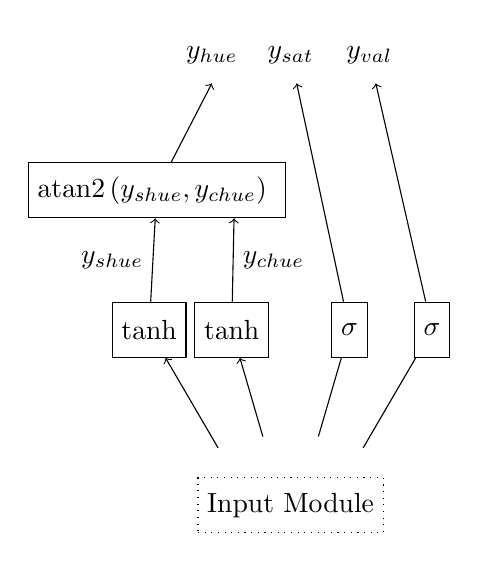
\begin{tikzpicture}
	
	\node (hiddenout)[layer, dotted]{Input Module};
	%\node (hiddenout)[above= 1 of input]{Affine with output width 4};
	%\draw[->](input) to (hiddenout);
	
	\node(outHue)[xshift=-1cm, above = 5 of hiddenout] {$y_{hue}$};
	\node(outSaturation)[above = 5 of hiddenout] {$y_{sat}$};
	\node(outValue)[xshift=1cm, above = 5 of hiddenout] {$y_{val}$};
	
	\node(Z)[above=-0.2cm of hiddenout.north]{};
	\node(Z2)[left=0cm of Z]{};%{$z_2$};
	\node(Z1)[left=0.3cm of Z2]{};%{$z_1$};
	\node(Z3)[right=0cm of Z]{};%{$z_3$};
	\node(Z4)[right=0.3cm of Z3]{};%{$z_4$};
	
	
	\node(s3)[layer, above=1 of Z3, xshift=0.5cm]{$\sigma$};
	\node(s4)[layer, above=1 of Z4, xshift=1cm]{$\sigma$};
	\draw[->](Z3) to (s3) to (outSaturation);
	\draw[->](Z4) to (s4) to (outValue);
	
	
	\node(AngHue)[layer, below = 1 of outHue, xshift=-0.7cm]{$ \mathrm{atan2} \left(y_{shue}, y_{chue} \right) $ };
	\draw[->](AngHue) to (outHue.south);
	
	\node(s1)[layer, above=1 of Z1, xshift=-1cm]{$\tanh$};
	\node(s2)[layer, above=1 of Z2, xshift=-0.5cm]{$\tanh$};
	\draw[->](Z1) to (s1);
	\draw[->](s1) to node[left]{$y_{shue}$} (AngHue);
	\draw[->](Z2) to (s2);
	\draw[->](s2) to node[right]{$y_{chue}$}  (AngHue.340);
	
	\end{tikzpicture}
	
	\caption{The Point Estimate Output Module.
		Here $\mathrm{atan2}$ is the quadrant preserving arctangent, outputting the angle in turns.
		\label{fig:pointoutmod}}
\end{figure}



\section{Evaluation}

\subsection{Perplexity in Color-Space}
Perplexity is a measure of how well the distribution, estimated by the model, matches the reality according to the observations in the test set.
Perplexity is commonly used for evaluating language models. Here however, it is being used to evaluate the discretized distribution estimate.
It can be loosely thought of as to how well the model's distribution does in terms of the size of an equivalent uniform distribution.
Note that this metric does not assume conditional independence of the color channels.

Here $\tau$ is the test-set made up of pairs consisting of a color name $t$, and a color-space point $\tilde{x}$;
and  $p(\tilde{x}\mid t)$ is the output of the evaluated model.
Perplexity is defined as:
\begin{equation}
PP(\tau{}) = \exptwo{\left(
	\frac{-1}{|\tau|} 
	\sum_{
		\forall(t,(\tilde{x})) \in \tau}
	\log_2 p(\tilde{x}\mid t)\right)}
\end{equation}

As the perplexity for a high-resolution discretized model will inherently be very large and difficult to read,
we define the standardized perplexity: $\frac{PP(\tau)}{n_{res}}$,
where $n_{res}$ is the total number of bins in the discretization scheme.
For all the results we present here $n_{res} = 256^3$.
This standardized perplexity gives the easily interpretable values \emph{usually} between zero and one.
It is equivalent to comparing the relative performance of the model to that of a uniform distribution of the same total resolution.
$\frac{PP(\tau)}{n_{res}}=1$ means that the result is equal to what we would see if we had distributed the probability mass uniformly into all bins in a 3D histogram.
$\frac{PP(\tau)}{n_{res}}=0.5$ means the result is twice as good as if we were to simply use a uniform distribution: it is equivalent to saying that the correct bin is selected as often as it would be had a uniform distribution with half as many bins been used (i.e. larger bins with twice the area).
The standardised perplexity is also invariant under different output resolutions.
Though for brevity we only  present results with 256 bins per channel, our preliminary results for using other resolutions are similar under standardized perplexity.

%\pdfcomment{Should mention cross entropy and KL divergence here? Closely related to perplexity}

\subsection{Angularly Correct Calculations on HSV}\label{sec:angularly-correct}
We use the HSV color-space \parencite{smith1978color} through-out this work.
In this format: hue, saturation and value all range between zero and one.
Note that we measure hue in \emph{turns}, rather than the more traditional degrees, or radians.
Having hue measured between zero and one, like the other channels, makes the modelling task more consistent.
Were the hue to range between $0$ and $2\pi$ (radians) or between $0$ and $360$ (degrees) it would be over-weighted in the loss function and evaluation metrics compared to the other channels.
This regular space means that errors on all channels can be considered equally.
Unlike many other colors spaces (CIELab, Luv etc.) the gamut is square and all combinations of values from the different channels correspond to realizable colors.


When performing calculations with the HSV color-space, it is important to take into account that hue is an angle.
As we are working with the color-space regularized to range between zero and one for all channels,
this means that a hue of one and a hue of zero are equivalent (as we measure in turns, in radians this would be $0$ and $2\pi$).

The square error of two hue values is thus calculated as:
\begin{equation}
SE(h_1, h_2) = \min \big( \left(h_1 - h_2 \right)^2, \, \left(h_1 - h_2 -1 \right)^2  \big)
\end{equation}
This takes into account that the error can be calculated clockwise or counter-clockwise; and should be the smaller.
Note that the $-1$ term is related to using units of turns, were we using radians it would be $-2\pi$


The mean of a set of hues ($\lbrace h_1,\,\ldots,\,h_N \rbrace$) is calculated as:
\begin{equation}
\bar h = \mathrm{atan2} \Bigg(%
	\frac{1}{N} \sum_{i=1}^{i=N} \sin (h_i), \,  %
	\frac{1}{N} \sum_{i=1}^{i=N} \cos (h_i)%
\Bigg)%
\end{equation}
This gives the mean angle.
%(Note again: as we measure angle in turns we use the turn trigonometric functions in implementation, though this mean is the same expression or any units).



\subsection{Operational Upper-bounds}
To establish a rough upper-limit on the modelling results we evaluate a direct method which bypasses the language understanding component of the task.
These direct methods do not process each term in the name:, they do not work with the language at all.
They simply map from the exact input text (no tokenization) to the pre-calculated distribution or mean of the training data for the exact color name.
This operational upper bound bypass the compositional language understanding part of the process.
It is as if the input module (as discussed in \Cref{sec:inputmod}) would perfectly resolve the sequence of terms into a single item.


They represent an approximate upper bound, as they fully exploit all information in the training data for each input.
There is no attempt to determine how each term affects the result.
We say approximate upper-bound, as it is not strictly impossible that the term-based methods may happen to model the test data better than can be directly determined by training data as processed per exact color name.
This would require learning how the terms in the color name combine in a way that exceeds the information directly present in the training data per class.
It is this capacity of learning how the terms combine that allow for the models to predict the outputs for combinations of terms that never occur in the training data (\Cref{sec:extrapodata}).
Doing this in a way that generalizes to get better results than the direct exploitation of the training data, would require very well calibrated control of (over/under)fitting.


\subsubsection{Operational Upper-bound for Distribution Estimation: KDE}\label{sec:direct-histogram} \label{sec:kernel-density-based-smoothing}
To determine an operational upper-bound for the distribution estimation tasks,
we use kernel-density estimation (KDE) in a formulation for non-parametric estimation \parencite{silverman1986density} .
The KDE effectively produces a smoothed histogram from the training data as processed in \Cref{sec:discretization}.
It causes adjacent bins to have most similar probabilities, thus matching to the mathematical notion of a continuous random variable.
This is applied on-top of the histogram used for the training data.
We use the Fast Fourier Transform (FFT) based KDE method of the \textcite{silverman1982algorithm}.
We use a Gaussian kernel, and select the bandwidth per color description based on leave-one-out cross validation on the training data.
A known issue with the FFT-based KDE method is that it has a wrap-around effect near the boundaries, where the mass that would be assigned outside the boundaries is instead assigned to the bin on the other side.
For the value and saturation channels we follow the standard solution of initially defining additional bins outside the true boundaries, then discarding those bins and rescaling the probability to one.
For the hue channel this wrap-around effect is exactly as desired.

In our evaluations using KDE rather than just the training histograms directly proved much more successful on all distribution estimation tasks.
This is because it avoids empty bins, and effectually interpolates probabilities between observations.
We found in preliminary investigations that using KDE-based method to be much better than add-one smoothing.

We also investigated the application of KDE to the training data,  before training our term-based neural network based distribution models.
Results for this can be found in \Cref{sec:smoothed-results}.
In brief, we found that smoothing the training data does not significantly affect the result of the neural network based models.
As discussed in \Cref{sec:quantitative-results}, this is because the neural networks are able to learn the smoothness relationship of adjacent bins.


Our KDE-based operational upper bound for distribution estimation bypasses the natural language understanding part of the task,
and directly uses the standard non-parametric probability estimation method to focus solely on modelling the distributions.
Matching its performance indicates that a model is effectively succeeding well at both the natural language understanding component and the distribution estimation component.


\subsubsection{Operational Upper-bound for Point Estimation: Mean-point}
In a similar approach, we also propose a method that directly produces a point estimate from a color name.
We define this by taking the mean of all the training observations for a given exact color name.
The mean is taken in the angularly correct way (as discussed in \Cref{sec:angularly-correct}).
Taking the mean of all the observations gives the theoretically optimal solution to minimize the squared error on the training data set.
As with our direct distribution estimation method, this bypasses the term based language understanding, and directly exploits the training data.
It thus represents an approximate upper bound on the point estimation performance of the term based models.
Though, as discussed in \Cref{sec:intro}, the notion of mean and of minimizing the square error is not necessarily the correct way to characterize selecting the optimal point estimate for colors.
It is however a consistent way to do so, and so we use it for our evaluations.



\subsection{Evaluation Strategies}

\subsubsection{Full Task}
We make use of the  Munroe dataset as prepared by \textcite{mcmahan2015bayesian} from the results of the XKCD color survey.
The XKCD color survey \parencite{Munroe2010XKCDdataset}, collected over 3.4 million observations from over 222,500 respondents.
McMahan and Stone take a subset from Munroe's full survey, by restricting it to the responses from native English speakers, 
and removing very rare color names with less than 100 uses.
This gives a total of 2,176,417 observations and 829 color names. 
They also define a standard test, development and train split.


\subsubsection{Unseen combination Task} \label{sec:extrapodata}
A primary interest in using the term based models is to be able to make predictions for never before seen descriptions of colors.
For example, based on the learned understanding of \texttt{salmon} and of \texttt{bright}, from examples like \texttt{bright green} and \texttt{bright red}, we wish for the system to make predictions about \texttt{bright salmon}, even though that description never occurs in the training data.
The ability to make predictions, such as these, illustrates term-based natural language understanding.
This cannot be done with the operational upper bound models, which by-passes the term processing step.
%
To evaluate this generalisation capacity, we define new sub-datasets for both testing and training.
We select the rarest 100 color descriptions from the full dataset,
with the restriction that every token in a selected description must still have at least 8 uses in other descriptions in the training set.
The selected examples include multi-token descriptions such as: \texttt{bright yellow green} and also single tokens that occur more commonly as modifiers than as stand-alone descriptions such as \texttt{pale}.

The unseen combination testing set has only observations from the full test set that do use those rare descriptions.
We define a corresponding restricted training set made up of the data from the full training set, excluding those  corresponding to the rare descriptions.
Similar restriction is done to create a restricted development set, so that no direct knowledge of the combined terms can leak during early-stopping.


By training on the restricted training set and testing on the unseen combination, we can assess the capacity of the models to make predictions for color descriptions not seen during training.
A similar approach was used in \textcite{acl2018WinnLighter} and in \textcite{DBLP:journals/corr/AtzmonBKGC16}.
We contrast this to the same models when trained on the full training set to see how much accuracy was lost.


\subsubsection{Order Task}
It is believed that the order of words in a color description matters, at least to some extent, for it's meaning.
For example, \natlang{greenish brown} and \natlang{brownish green} are distinct, if similar, colors.
To assess the models on their ability to make predictions when order matters we construct the order test set.
This is a subset of the full test set containing only descriptions with terms that occur in multiple different orders.
There are 76 such descriptions in the full dataset.
Each of which has exactly one alternate ordering.
This is unsurprising as while color descriptions may have more than 2 terms, normally one or more of the terms is a joining token such as \natlang{ish} or \natlang{-}.
We only construct an order testing set, and not a corresponding training set, as this is an evaluation using the model trained on the full training data.




\section{Experimental Setup}

\subsection{Implementation}
The implementation of all the models was in the julia programming language \parencite{Julia}.
The full implementation can be downloaded from the GitHub repository.\footnote{Implementation source is at \url{https://github.com/oxinabox/ColoringNames.jl}}
The machine learning components make heavy use of the MLDataUtils.jl\footnote{MLDataUtils.jl is available from \url{https://github.com/JuliaML/MLDataUtils.jl}} and TensorFlow.jl,\footnote{TensorFlow.jl is available from \url{https://github.com/malmaud/TensorFlow.jl}} packages.
The latter of which we enhanced significantly to allow for this work to be carried out.
The discretization and the KDE for the Operational Upper Bound is done using KernalDensityEstimation.jl.%
\footnote{KernalDensityEstimation.jl  is available from \url{https://github.com/JuliaStats/KernelDensity.jl}}
% TODO: If DataDeps paper available before this one, cite it here.

\subsection{Common Network Features}
Drop-out\parencite{srivastava2014dropout}  is used on all ReLU layers and on the GRU in the RNN, with threshold of 0.5 during training.
The network is optimized using Adam \parencite{kingma2014adam}, and a learning rate of 0.001.
Early stopping is checked every 10 epochs using the development dataset.
Distribution estimation methods are trained using the full batch (where each observation is a distribution) for every epoch.
Point Estimation methods are trained using randomized mini-batches of $2^{16}$ observations (which are each color-space triples).
All hidden-layers, except as otherwise precluded (inside the convolution, and in the penultimate layer of the point estimation networks) have the same width 300, as does the embedding layer.



\section{Results}\label{sec:results}


\documentclass[11pt,a4paper]{article}
%\usepackage[author={Lyndon}]{pdfcomment}

\usepackage{booktabs}
\usepackage{tikz}
\usepackage{graphicx}
\usepackage[space]{grffile}


\begin{document}
\def\maincolors{%
	brown-orange,
	orange-brown,	
	yellow-orange,
	orange-yellow,
	brownish green,
	greenish brown,
	bluish grey,
	greyish blue,
	pink-purple,
	purple-pink,
	green,
	greenish,
	purple,	
	purplish,
	brown,
	brownish,
	black,
	grey,
	white%
}

\def\oovcolors{
	%	brownish 1Green,
	%	bluish gray,
	1Brown,
	1Green,
	1Purple,
	gray,
	1Gray%
}


\tikzset{lastline/.style={opacity=1}}
\newcommand{\distfigs}[2]{
	\begin{tikzpicture}[defaultfig]%
	\foreach[count=\mdlii from 0] \mdlfile/\mdlname in #1 {%
		\node at (3.1*\mdlii cm, -1cm) {\sffamily \mdlname};%
		\foreach[count=\colii from 0] \colorname in #2 {%
			\xdef\topy{1.1*\colii}
			\node at (3.1*\mdlii cm, \topy cm) %
			{\includegraphics[height=0.95cm]{%
					figs/demo/dist/\mdlfile/\colorname}%
			};%

		}%
		\xdef\topy{\topy+1}
		\node at (3.1*\mdlii cm, -1cm) {\sffamily \mdlname};%
		\node at (3.1*\mdlii cm, \topy) {\sffamily \mdlname};%
	}%
	%

%	\draw[dashed] (1.555, -1.1) -- (1.555, \topy);%
%	\draw[lastline] (3*1.555,-1.1) -- (3*1.555, \topy);%
%	\draw[dashed,lastline] (5*1.555,-1.1) -- (5*1.555, \topy);%
	%
	\end{tikzpicture}%
}%

\subsection{Qualitative Results}\label{sec:qualitative-results}

\newcommand{\pointfigs}[3]{
	\begin{tikzpicture}%
	\foreach[count=\mdlii from 0] \mdlfile/\mdlname in #1 {%
		\node(fig\mdlfile) at (3.1*\mdlii cm, 0) %
		{\includegraphics[height=#3 cm]{%
				figs/demo/point/\mdlfile/#2}%
		};%
		\node[below = -0.7 of fig\mdlfile] {\sffamily \mdlname};%
		\node[above = -0.75 of fig\mdlfile] {\sffamily \mdlname};%
	}%
	\end{tikzpicture}%
}%


\begin{figure}
	\resizebox{\textwidth}{!}{
		\distfigs{{Direct/{Training Data}, Direct-smoothed/{\shortstack{Non-compositional\\ Baseline}}, SOWE/SOWE, CNN/CNN, GRU/GRU, LSTM/LSTM}}{\maincolors}
	%\distfigs{{Direct/{Training Data}, Direct-smoothed/{\shortstack{Non-compositional\\ Baseline}}, GRU/GRU, LSTM/LSTM}}{\maincolors}
	}
	\caption{Some examples of the output distribution estimates from the models trained on the full dataset} \label{fig:distout1}
\end{figure}

\begin{figure}
	\resizebox{\textwidth}{!}{
		\pointfigs{{Direct/{\shortstack{Non-compositional\\ Baseline}}, SOWE/SOWE, CNN/CNN, GRU/GRU, LSTM/LSTM}}{maincolors}{18}
	}
	\caption{Some examples of the output point estimates from the models trained on the full dataset} \label{fig:pointout}
\end{figure}


To get an understanding of the problem and how the models are performing, we consider some of the outputs of the model for particular cases.
\Cref{fig:distout1} shows examples of distribution estimates, and 
\Cref{fig:pointout} shows similar examples for point estimates.
Both  are  taken  from models trained on  the full training dataset.
It can be seen that the models' outputs using term based estimation are generally similar to the non-term-based \empmodel{}, as is intended.
This shows that the models are correctly fitting to estimate the colors.
It can be noted  that  in general the  colors  are  very good, with  only a few marked exceptions,   discussed in the  following sections, particularly around multi-word colors.
To  the naked  eye,  it is hard to to distinguish  between the outputs of the different models.
The general high quality of the estimates aligns with the strong results found in the quantitative evaluations discussed in \Cref{sec:quantitative-results}.
The example shown  in \Cref{fig:distout1,fig:pointout} serve  to indicate that while the  quantitative results do show that some of the models perform better than  others, the  true visual difference is very small.

\subsubsection{On the effects of word-order}
The different input modules have a different capacity to leverage word-order.
This is reflected in \Cref{fig:distout1,fig:pointout},
when considering the pairs of outputs that differ only in word order, such as \natlang{purple-pink} and \natlang{pink-purple}.
The plots presented for the training data and for the \empmodel{} show that such color name pairs are subtly different but similar.
The SOWE model is unable to take into account word order at all, and so produces identical outputs for all orders.
The CNN models produce very similar outputs but not strictly identical -- spotting the difference requires a very close observation.
This is in-line with the different filter sizes allowing the CNN to effectively use n-gram features, and finding that the unigram features are the most useful.
Both RNN models (GRU and LSTM) produce estimated distributions that visibly depend on the order of words.
It seems that the first term dominates the final output: for example \natlang{greenish brown} is more green, and  \natlang{brownish green} is more brown, contrary to the linguistic understanding.
The RNN outputs are more similar to the color described by first term than any later terms.
We can see that the first term is not solely responsible for the final output however, as \natlang{purple-pink}, \natlang{purple} and \natlang{purplish} (tokenized as \natlang{purple}, \natlang{ish}) are all different.
It is surprising that the RNNs outputs  are dominated by the first term and not the latter terms\footnote{So much so that we double checked our implementation to be sure that it wasn't processing the inputs backwards.}.
This shows that they are  functioning to remember the earlier inputs.
However, they are struggling to attribute the significance of the word order.
Linguistically we would expect the last term to be the most significant:
\natlang{greenish brown} is a shade of brown, not green.
This expectation is reflected in the histogram for the training data.
Although, for many of the order swapped colors the training histograms shown are very similar regardless of the order.



\subsubsection{On the smoothness of the distribution estimates}\label{sec:learnedsmoothness}
In \Cref{fig:distout1} it can be seen that the term-based distribution estimation models are much smoother than the corresponding histograms taken from the  training data.
They are not as smooth as the \empmodel{} which explicitly uses KDE.
However, they are much smoother than would be expected, had the output bins been treated independently.
Thus it is clear that the models are learning that adjacent bins should have similar output values.
This is a common feature of all the training data, no matter which color is being described.
This learned effect is in line with the fact that color is continuous, and is only being represented here as discrete.
We note in relation to this learned smoothness: that while the models capture the highly asymmetrical shapes of most distributions well, they do not do well at capturing small dips.
Larger multi-modes as seen in the achromatic colors such as \natlang{white}, \natlang{grey}, \natlang{black}, \natlang{white}, are captured; but smaller dips such as the hue of \natlang{greenish} being more likely to be on either side of the green spectrum are largely filled in.
In general, it seems clear that additional smoothing of the training data is not required for the neural network based models.
This aligns with the results presented in \Cref{sec:smoothed-results}.




%%%%%%%%%%%%%%%%%%%%%%%%%%%%%%%%%%%%%%%%%%%%%%%%%%%%%%%%%%%



\end{document}
\input{pubColorEst-quantres.tex}


\subsection{Completely Unseen Color Estimation From Embeddings}\label{sec:embeddingonly}
As an interesting demonstration of how the models function by learning the transformation from the embedding space to the output ,we briefly consider the outputs for color-names that do not occur in the training or testing data at all.
This is even more extreme than the unseen combination task considered in \Cref{tbl:distextrapo,tbl:pointextrapo} where the terms appeared in training, but not the combination of terms.
In the examples shown in \Cref{fig:oovdist,fig:oovpoint}, where the terms never occurred in the training data at all, our models exploit the fact that they work by transforming the word-embedding space to predict the colors.
There is no equivalent for this in the direct models.
While \natlang{Grey} and \natlang{gray} never occur in the training data; \natlang{grey} does, and it is near-by in the word-embedding space.
Similar is true for the other colors that vary by capitalization.
We only present a few examples of single term colors here, and no quantitative investigation, as this is merely a matter of interest.

It is particularly interesting to note that the all the models make similar estimations for each color.
This occurs both for point estimation and for distribution estimation.
They do well on the same colors and make similar mistakes on the colors they do poorly at.
The saturation of \natlang{Gray} is estimated too high, making it appear too blue/purple, this is also true of \natlang{grey} though to a much lesser extent.
\natlang{Purple} and \natlang{Green} produce generally reasonable estimates.
The hue for \natlang{Brown} is estimated as having too much variance, allowing the color to swing into the red or yellowish-green parts of the spectrum.
This suggests that in general all models are learning a more generally similar transformation of the space.
In general the overall quality of each model seems to be in line with that found in the results for the full tests.


\begin{figure}
	\distfigs{{SOWE/SOWE, CNN/CNN, RNN/RNN}}{\oovcolors}	
	\caption{Some example distribution estimations for colors names which are completely outside the training data. The terms: \natlang{Brown}, \natlang{gray}, \natlang{Gray}, \natlang{Green}, and \natlang{Purple}, do not occur in any of the color data; however \natlang{brown}, \natlang{grey} \natlang{green}, and \natlang{purple} do occur.} \label{fig:oovdist}
\end{figure}

\begin{figure}
	\pointfigs{{SOWE/SOWE, CNN/CNN, RNN/RNN}}{oovcolors}{5}
	\caption{Some example point estimates for colors names which are completely outside the training data. The terms: \natlang{Brown}, \natlang{gray}, \natlang{Gray}, \natlang{Green}, and \natlang{Purple}, do not occur in any of the color data; however \natlang{brown}, \natlang{grey} \natlang{green}, and \natlang{purple} do occur.} \label{fig:oovpoint}
\end{figure}



\section{Conclusion}
We have presented three input modules (SOWE, CNN, RNN),
and two output modules (distribution estimate, and point estimate)
that are suitable for using machine learning to make estimates about color based on the terms making up its name.
We contrasted these to an operational upper bound model for each task which bypassed the term-wise natural language understanding component of the problem.
We found the results for SOWE, and CNN were very strong, approaching this upper bound.


A key take away from our results is that using a SOWE should be preferred over an RNN for short phrase natural language understanding tasks when order is not a very significant factor.
The RNN is the standard type of model for problems with sequential input, such as color names made up of multiple words as we considered here.
However, we find its performance to be significantly exceeded by the SOWE and CNN.
The SOWE is an unordered model roughly corresponding to a bag of words.
The CNN similarly roughly correspondents to a bag of ngrams, in our case a bag of all 1,2,3,4 and 5-grams.
This means the CNN can readily take advantage of both fully ordered information, using the filters of length 5, down to unordered information using  filters of length 1.
The RNN however must fully process the ordered nature of its inputs, as its output comes only from the final node.
It would be interesting to further contrast a bidirectional RNN.

In a broader context, we envisage the distribution learned for a color name can be used as a prior probability and when combining with additional context information, this can be used for better prediction in areas such as document classification and sentiment detection.

A further interesting avenue for investigation would condition the model not only on the words used but also on the speaker.
The original source of the data \textcite{Munroe2010XKCDdataset}, includes some demographic information which is not exploited by any known methods.
It is expected that color-term usage may vary with subcultures.


\clearpage
\input{pubColorEst-supp.tex}


}
%\end{document}
